\chapter{Special Relativity: Velocity Composition, Proper Interval, and Four-Vectors}

We return, just as the lecture does, to the one-dimensional railroad track. Last time the Lorentz transformation was derived; now Susskind reopens the picture, reminds us what the symbols mean, and then presses them harder. These notes follow Leonard Susskind's lecture, with transcript and frame curation prepared by LazyingArt LLC and Video2Book. The argument unfolds in three stages: first we reread the Lorentz transformation geometrically, then we compose two boosts and discover the relativistic law of velocity addition, and finally we step back to the invariant interval and reorganize the discussion in the language of four-vectors.

\section{Recap: Two Frames, One Axis, and the Choice \(c=1\)}

The lecture begins by saying explicitly what was implicit before: we are considering motion along a single axis. One should picture a long railroad track, stationary observers at the station, and other observers riding in the train. The two coordinate systems are not abstract labels; they are operational systems built from meter sticks and clocks at rest in their respective frames.

The basic postulate remains Einstein's. Every inertial observer assigns the same speed to light. In the units used through most of the lecture, that speed is
\begin{equation}
c=1.
\end{equation}
This is only a choice of units. We may work in seconds and light-seconds, or in years and light-years, so that velocities become dimensionless fractions of the speed of light. Whenever we want to go back to conventional units, we restore factors of \(c\) by dimensional consistency. That is the rule Susskind emphasizes.

Now let an event occur, perhaps a flash bulb going off somewhere in the train. The stationary observer assigns coordinates \((x,t)\), while the observer in the train assigns \((x',t')\). The Lorentz transformations are
\begin{align}
x' &= \frac{x-vt}{\sqrt{1-v^2}},
&
t' &= \frac{t-vx}{\sqrt{1-v^2}}.
\end{align}
They may be inverted without any new idea:
\begin{align}
x &= \frac{x'+vt'}{\sqrt{1-v^2}},
&
t &= \frac{t'+vx'}{\sqrt{1-v^2}}.
\end{align}
The two frames are related reciprocally; the only asymmetry is the sign of the relative velocity when we describe one frame from the other. For boosts along the \(x\)-axis, the transverse directions are unaffected:
\begin{equation}
y'=y,
\qquad
z'=z.
\end{equation}

The lecture is careful about what these equations mean. They relate coordinate assignments to the same event. Each observer uses rods and clocks at rest relative to himself, and the transformation tells us how those coordinate assignments correlate.

\section{Reading Motion Off the Lorentz Transformation}

At this point Susskind makes a very simple but very instructive move. He asks us not to stare at the whole formula, but to ask what it says about the origin of the primed frame. The primed observer is at rest in his own coordinates, so his position is characterized by
\begin{equation}
x'=0.
\end{equation}
Therefore, from the space transformation,
\begin{equation}
x'=0
\qquad\Longleftrightarrow\qquad
x-vt=0
\qquad\Longleftrightarrow\qquad
x=vt.
\end{equation}
The denominator does not matter for this purpose. To locate the line \(x'=0\), we only need the numerator. So the worldline of the origin of the primed coordinates, described in the unprimed frame, is \(x=vt\). That is how we read the relative velocity directly from the transformation.

\begin{figure}[t]
\centering

\includegraphics[width=0.78\textwidth]{lecture_02_figure_02.png}
\caption{Board sketch used when the lecture identifies the primed origin inside the train. The secure visible labels are the unprimed frame \(x,t\) and the condition \(x'=0\).}
\end{figure}

This board drawing is not a spacetime diagram in the analytic sense. It is a cartoon of the situation: the train is drawn as a box, the passenger sits inside it, the station observer is below, and a dashed line ties a marked event in the train to a marked location on the stationary line. The nearby primed event label is not fully legible, but the point of the picture is clear enough: the origin of the primed frame occupies a definite place in the train, and in the unprimed description that place moves according to \(x=vt\).

\begin{figure}[t]
\centering
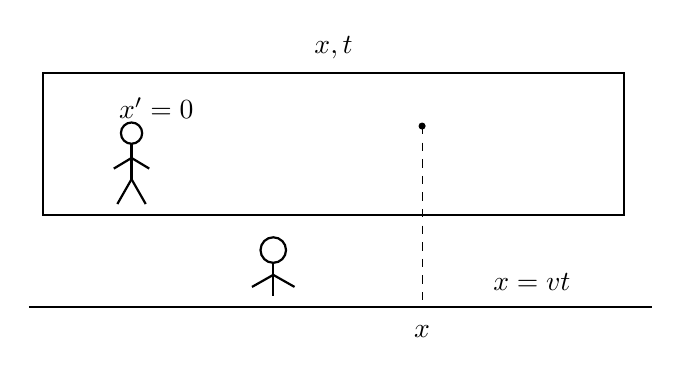
\begin{tikzpicture}[scale=0.9]
\draw[thick] (0,2.2) rectangle (8.2,4.2);
\draw (4.1,4.55) node {$x,t$};

\draw[thick] (-0.2,0.9) -- (8.6,0.9);

\draw[thick] (1.25,3.35) circle (0.15);
\draw[thick] (1.25,3.2) -- (1.25,2.7);
\draw[thick] (1.25,3.0) -- (1.0,2.85);
\draw[thick] (1.25,3.0) -- (1.5,2.85);
\draw[thick] (1.25,2.7) -- (1.05,2.35);
\draw[thick] (1.25,2.7) -- (1.45,2.35);
\draw (1.6,3.7) node {$x'=0$};

\fill (5.35,3.45) circle (0.05);
\draw[dashed] (5.35,3.45) -- (5.35,0.9);

\draw[thick] (3.25,1.7) circle (0.18);
\draw[thick] (3.25,1.52) -- (3.25,1.05);
\draw[thick] (3.25,1.35) -- (2.95,1.18);
\draw[thick] (3.25,1.35) -- (3.55,1.18);

\draw (5.35,0.55) node {$x$};
\draw (6.9,1.25) node {$x=vt$};
\end{tikzpicture}
\caption{Cleaned schematic of the same idea. The lecture's claim is modest and precise: the primed origin is the line \(x'=0\), and in the unprimed frame that line is \(x=vt\).}
\end{figure}

\section{A Third Observer: The Kiddie Car and the Composition of Boosts}

Now the lecture pivots: ``now we want to do another exercise.'' Inside the train there is a third observer, a child in a kiddie car. The train frame still uses coordinates \((x',t')\), but the child now has his own rods and clocks and therefore his own coordinates \((x'',t'')\). The train moves with speed \(v\) relative to the station, the kiddie car moves with speed \(u\) relative to the train, and the question is this:

What speed does the stationary observer assign to the kiddie car?

Susskind is explicit that he does not know how to guess the answer. So he names the unknown velocity \(w\) and sets up the calculation. Between the primed and double-primed frames, the Lorentz transformation has the same form as before:
\begin{align}
x'' &= \frac{x'-ut'}{\sqrt{1-u^2}},
&
t'' &= \frac{t'-ux'}{\sqrt{1-u^2}}.
\end{align}

\begin{figure}[t]
\centering

\includegraphics[width=0.58\textwidth]{lecture_02_figure_03.png}
\caption{The composition-of-boosts setup on the board. The lecture first writes the ordinary Lorentz transformation and then a second one from primed to double-primed variables. The board mixes \(X\) and \(x\); we standardize to lowercase \(x\).}
\end{figure}

The lecture then narrows its attention. ``Let's focus on the space equation.'' We know \(x'\) and \(t'\) in terms of \(x\) and \(t\), so we simply substitute:
\begin{align}
x''
&= \frac{x'-ut'}{\sqrt{1-u^2}} \\
&= \frac{1}{\sqrt{1-u^2}}
\left[
\frac{x-vt}{\sqrt{1-v^2}}
-
u\frac{t-vx}{\sqrt{1-v^2}}
\right] \\
&= \frac{(x-vt)-u(t-vx)}{\sqrt{1-v^2}\sqrt{1-u^2}} \\
&= \frac{(1+uv)x-(u+v)t}{\sqrt{1-v^2}\sqrt{1-u^2}}.
\end{align}
The denominator is the product of the two square roots. Susskind deliberately does not dwell on it. The numerator is the part that tells us the story. Just as before, we locate the origin of the moving frame by setting its spatial coordinate equal to zero:
\begin{equation}
x''=0.
\end{equation}
That means the numerator must vanish:
\begin{equation}
(1+uv)x-(u+v)t=0.
\end{equation}
So the worldline of the double-primed origin in the station frame is
\begin{equation}
x=\frac{u+v}{1+uv}\,t.
\end{equation}
And from that worldline we read off the velocity:
\begin{equation}
w=\frac{u+v}{1+uv}.
\end{equation}

This is the payoff. The stationary observer does not see the kiddie car move with velocity \(u+v\). He sees it move with the relativistically corrected velocity \(w\). After a brief correction on the board, the composed transformation may be written in the cleaned standard form
\begin{align}
x'' &= \frac{x-wt}{\sqrt{1-w^2}},
&
t'' &= \frac{t-wx}{\sqrt{1-w^2}},
\end{align}
where \(w\) is exactly the composed velocity above.

\begin{figure}[t]
\centering

\includegraphics[width=0.78\textwidth]{lecture_02_figure_04.png}
\caption{The later board sketch makes the geometric point explicit. Susskind points to the double-primed location and says that this corresponds to \(x''=0\).}
\end{figure}

\begin{figure}[t]
\centering
\begin{tikzpicture}[scale=0.9]
\draw[thick] (0,2.25) rectangle (9.1,4.25);
\draw (4.55,4.6) node {$x,t$};

\draw[thick] (-0.2,0.95) -- (9.4,0.95);

\draw[thick] (1.25,3.35) circle (0.15);
\draw[thick] (1.25,3.2) -- (1.25,2.75);
\draw[thick] (1.25,3.0) -- (1.0,2.85);
\draw[thick] (1.25,3.0) -- (1.5,2.85);
\draw[thick] (1.25,2.75) -- (1.05,2.35);
\draw[thick] (1.25,2.75) -- (1.45,2.35);
\draw (1.65,3.7) node {$x'=0$};

\fill (5.4,3.45) circle (0.05);
\draw[dashed] (5.4,3.45) -- (5.4,0.95);

\draw[thick] (6.1,2.85) -- (7.2,2.85);
\draw[thick] (6.35,2.85) -- (6.5,3.1);
\draw[thick] (6.55,2.85) -- (6.7,3.1);
\draw[thick] (6.8,2.85) -- (6.95,3.1);
\draw[thick] (6.3,2.85) circle (0.13);
\draw[thick] (7.0,2.85) circle (0.13);
\draw (6.75,3.42) node {$x''=0$};

\draw[->,thick] (7.35,3.0) -- (8.45,3.0);
\draw (8.65,3.0) node {$u$};

\draw[->,thick] (6.0,1.35) -- (8.1,1.35);
\draw (8.35,1.35) node {$w$};

\draw (6.45,0.55) node {$x=\dfrac{u+v}{1+uv}\,t$};
\end{tikzpicture}
\caption{Cleaned version of the three-frame cartoon. The upper arrow is the velocity \(u\) measured in the train frame, and the lower arrow is the resulting velocity \(w\) measured in the station frame.}
\end{figure}

The lecture immediately raises the dimensional question. In relativistic units the formula is
\begin{equation}
w=\frac{u+v}{1+uv},
\end{equation}
but in conventional units the denominator cannot remain \(1+uv\); it must be dimensionless. So the restored formula is
\begin{equation}
w=\frac{u+v}{1+\dfrac{uv}{c^2}}.
\end{equation}
This is the unique restoration by dimensional consistency.

We can now compare Einstein with Newton. Newton would have said simply
\begin{equation}
w_{\mathrm{Newton}}=u+v.
\end{equation}
Relativity modifies this by the denominator. If \(u\) and \(v\) are both small compared with \(c\), then \(uv/c^2\) is tiny and
\begin{equation}
w\approx u+v.
\end{equation}
So the Newtonian rule survives as an approximation.

Susskind then tests the formula. If \(u=v=0.01\), meaning each speed is one percent of the speed of light, then
\begin{equation}
w=\frac{0.02}{1+0.0001},
\end{equation}
which is only a hair smaller than \(0.02\). But if \(u=v=0.9\), then
\begin{equation}
w=\frac{0.9+0.9}{1+0.9^2}=\frac{1.8}{1.81}<1.
\end{equation}
Newton would have predicted \(1.8\), faster than light. The relativistic correction prevents that. This is exactly the protective feature the lecture wants us to notice: composing subluminal motions does not produce a superluminal result.

\subsection{Question \& Answer}

\paragraph{Question.} Suppose the child does not pedal a kiddie car at all, but sends a beam of light forward. Why do both frames still say that the beam moves with speed \(1\)?

\paragraph{Answer.} In the addition formula we simply set the speed in the train frame equal to the speed of light:
\begin{equation}
u=1.
\end{equation}
Then
\begin{equation}
w=\frac{1+v}{1+v}=1.
\end{equation}
So a light ray remains a light ray under the composition of boosts. This is not an extra theorem sitting on top of the Lorentz transformation. It is the property around which the whole structure was built.

\section{Question \& Answer: Why Glass Walls Do Not Settle the Matter}

The lecture now pauses for an audience objection. If the train had glass walls, could not the station observer simply look through them and watch both the passenger and the kiddie car at once?

\subsection{Question \& Answer}

\paragraph{Question.} Why is that not the right way to think about the problem?

\paragraph{Answer.} Because the issue is not what the eye sees. The issue is how events are assigned coordinates by rods and clocks at rest in a frame. Raw visual appearance mixes in the travel time of light from the event to the observer, and that is a more complicated question. What relativity is organizing here is the correlation of measured positions and times in inertial frames.

This is a small but essential correction of instinct. If we let ourselves drift from coordinate measurement back into naive appearance, we smuggle simultaneity problems back in through the side door. Susskind cuts that off sharply. The transformation laws are universal. They do not depend on whether the train walls are glass.

\section{Proper Interval, Extra Spatial Directions, and the Light Cone}

With the velocity-addition story complete, the lecture changes scale. ``The next thing we talked about last time'' was the proper interval, and now that idea is recalled and extended.

In one space dimension and one time dimension, the invariant is
\begin{equation}
\tau^2=t^2-x^2.
\end{equation}
Its importance is that every inertial observer agrees on it:
\begin{equation}
\tau^2=t^2-x^2=t'^2-x'^2=t''^2-x''^2.
\end{equation}
The coordinates themselves are frame-dependent, but this combination is not. It is the proper interval between the two events. If a clock moves from one event to the other, the time it reads is the proper time associated with that interval.

Now the lecture reinstates the other spatial directions. This is done in a concrete and almost Euclidean way. Once we allow rotations of the spatial axes, \(x^2\) is recognized as only part of the square of the spatial distance from the origin. By Pythagoras,
\begin{equation}
x^2 \longrightarrow x^2+y^2+z^2.
\end{equation}
Therefore the invariant interval in \(3+1\) dimensions becomes
\begin{equation}
\tau^2=t^2-x^2-y^2-z^2.
\end{equation}
This is the central invariant of special relativity. In ordinary Euclidean geometry the invariant under rotations is the distance squared from the origin. Here the invariant is a different kind of squared distance, one in which time and space enter with opposite signs.

Light rays are then characterized by a null interval. In \(1+1\) dimensions, a light ray moving to the right satisfies \(x=t\), while one moving to the left satisfies \(x=-t\). In either case,
\begin{equation}
t^2-x^2=0.
\end{equation}
In \(3+1\) dimensions the same statement becomes
\begin{equation}
t^2-x^2-y^2-z^2=0.
\end{equation}
So photons move on trajectories for which the proper interval vanishes.

\begin{figure}[t]
\centering
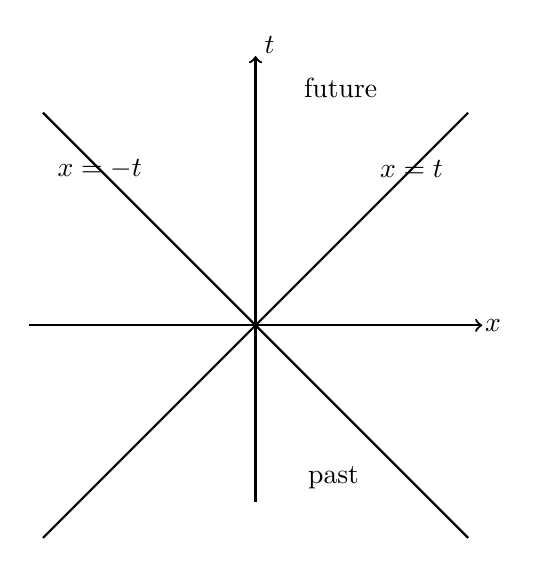
\begin{tikzpicture}[scale=0.9]
\draw[->,thick] (-3.2,0) -- (3.2,0);
\draw[->,thick] (0,-2.5) -- (0,3.8);
\draw (3.35,0) node {$x$};
\draw (0.2,3.95) node {$t$};

\draw[thick] (0,0) -- (3,3);
\draw[thick] (0,0) -- (-3,3);
\draw[thick] (0,0) -- (3,-3);
\draw[thick] (0,0) -- (-3,-3);

\draw (2.2,2.2) node {$x=t$};
\draw (-2.2,2.2) node {$x=-t$};
\draw (1.2,3.35) node {future};
\draw (1.1,-2.15) node {past};
\end{tikzpicture}
\hspace{1cm}
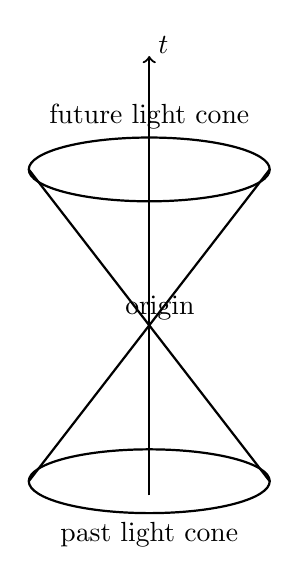
\begin{tikzpicture}[scale=0.9]
\draw[->,thick] (0,-2.4) -- (0,3.8);
\draw (0.2,3.95) node {$t$};

\draw[thick] (0,0) -- (-1.7,2.2);
\draw[thick] (0,0) -- (1.7,2.2);
\draw[thick] (0,0) -- (-1.7,-2.2);
\draw[thick] (0,0) -- (1.7,-2.2);

\draw[thick] (0,2.2) ellipse (1.7 and 0.45);
\draw[thick] (0,-2.2) ellipse (1.7 and 0.45);

\draw (0,2.95) node {future light cone};
\draw (0,-2.95) node {past light cone};
\draw (0.15,0.25) node {origin};
\end{tikzpicture}
\caption{On the left, the \(1+1\)-dimensional light cone appears as \(45^\circ\) null lines. On the right is the lecture's schematic higher-dimensional cone picture.}
\end{figure}

This gives the usual terminology. The future light cone is the set of points that can be reached by light emitted from the origin. The past light cone is the set of points from which light can be sent to the origin. In the lecture, the terminology is introduced lightly; what matters is the null condition that defines these sets.

\subsection{Question \& Answer}

\paragraph{Question.} If relativity has the invariant \(\tau^2=t^2-x^2-y^2-z^2\), what is the corresponding invariant in Newtonian mechanics?

\paragraph{Answer.} Just the time interval. Newtonian mechanics keeps \(\Delta t\) fixed for all inertial observers. Relativity gives up that universal time and replaces it with an invariant spacetime interval.

\section{From Ordinary Vectors to Four-Vectors}

Only now does the lecture turn to condensed notation. The order matters. We do not begin with abstract symbols and then search for an interpretation; we begin with the geometry and only then compress it.

The most primitive example of a vector in ordinary space is the interval between two points. If we move the tail of the vector to the origin, the vector is specified by three coordinates. We may write them as
\begin{equation}
x^i=(x,y,z),
\qquad i=1,2,3.
\end{equation}
Here the index \(i\) runs only over spatial directions.

But for spacetime we need one more coordinate: the time at which the event occurs. So we enlarge the vector to a four-component object,
\begin{equation}
x^\mu=(t,x,y,z),
\qquad \mu=0,1,2,3.
\end{equation}
The historical convention used in the lecture is that time is the zeroth component:
\begin{equation}
x^0=t,
\qquad
x^1=x,
\qquad
x^2=y,
\qquad
x^3=z.
\end{equation}
With this notation, the interval is written compactly as
\begin{equation}
\tau^2=(x^0)^2-(x^1)^2-(x^2)^2-(x^3)^2.
\end{equation}

Susskind is careful here: this is mostly notation. There is ``no content'' in the relabeling itself. The content is that Lorentz transformations act linearly on these four components, just as ordinary rotations act linearly on spatial vectors. So one may represent a Lorentz transformation by a matrix acting on a column vector. The point of the notation is not ornament. It is to organize the physics in a way that will be useful when we turn to dynamics.

\section{Small Intervals and Four-Velocity}

The lecture ends by changing from finite positions to small intervals along a trajectory. Instead of taking the coordinates of a point relative to an origin, we take a short displacement along a worldline:
\begin{equation}
\Delta x^\mu=(\Delta t,\Delta x,\Delta y,\Delta z).
\end{equation}
Susskind says explicitly: when you hear ``small,'' think calculus. But for the moment the interval is still treated discretely. The associated invariant proper-time interval is
\begin{equation}
\Delta\tau^2=\Delta t^2-\Delta x_i\Delta x_i
=\Delta t^2-\Delta x^2-\Delta y^2-\Delta z^2.
\end{equation}

Now compare this with ordinary velocity. In ordinary mechanics we divide a small spatial displacement by \(\Delta t\), and we obtain a three-component velocity. Here we divide the spacetime displacement by the invariant interval:
\begin{equation}
u^\mu=\frac{\Delta x^\mu}{\Delta\tau}.
\end{equation}
This is the four-velocity. It has four components, and the lecture deliberately labels it with \(u^\mu\) rather than \(v^\mu\). If we pass to continuum notation, the same object becomes
\begin{equation}
u^\mu=\frac{dx^\mu}{d\tau}.
\end{equation}

\begin{figure}[t]
\centering
\begin{tikzpicture}[scale=0.95]
\draw[->,thick] (-0.2,0) -- (4.8,0);
\draw[->,thick] (0,-0.2) -- (0,4.8);
\draw (4.95,0) node {$x$};
\draw (0.2,4.95) node {$t$};

\draw[thick] (0.5,0.5) .. controls (1.2,1.1) and (1.8,2.0) .. (2.5,2.8)
             .. controls (3.0,3.35) and (3.45,3.75) .. (4.1,4.2);

\draw[thick] (2.38,2.66) -- (2.92,3.18);
\draw (3.45,3.25) node {$\Delta x^\mu$};
\draw (2.05,2.12) node {$\Delta\tau$};
\end{tikzpicture}
\caption{A short segment along a worldline. In the lecture this interval is introduced first as a discrete \(\Delta x^\mu\), with the differential version postponed only slightly.}
\end{figure}

And then the lecture stops, at exactly the right place. The next question is how this four-velocity relates to the ordinary three-velocity, but that question is deliberately left hanging for the next meeting. The reason is clear from the closing lines: we are heading toward a relativistic theory of the motion of particles, toward relativistic momentum, energy, acceleration, and ultimately a generalization of \(F=ma\). Four-vectors are the language in which that theory will be written.

\section{Summary}

The lecture unfolds in a clean sequence. We first return to the train and station and remind ourselves what the Lorentz transformation means operationally. Then we read the motion of the primed origin directly from the condition \(x'=0\), obtaining the worldline \(x=vt\). That same trick is then repeated for a third observer in the kiddie car. By composing two Lorentz transformations and setting \(x''=0\), we arrive at the relativistic velocity-addition law
\begin{equation}
w=\frac{u+v}{1+uv},
\end{equation}
or, with ordinary dimensions restored,
\begin{equation}
w=\frac{u+v}{1+\dfrac{uv}{c^2}}.
\end{equation}

Having done that calculation, the lecture returns to the deeper invariant structure:
\begin{equation}
\tau^2=t^2-x^2-y^2-z^2.
\end{equation}
Light rays are null, \(\tau^2=0\), and the future and past light cones are the geometric expression of that fact. Finally, the whole discussion is compressed into four-vector notation, ending with the definition
\begin{equation}
u^\mu=\frac{\Delta x^\mu}{\Delta\tau},
\end{equation}
which points directly toward relativistic particle dynamics. The chapter therefore ends where the lecture ends: with the sense that the real mechanics is about to begin.